% tADRguide.tex
% v1.0 released January 2013

\documentclass{tADR2e}

\usepackage{graphicx}
\usepackage{subfloat}
\usepackage{subfigure}
\usepackage{subfig}
\usepackage{color}
\usepackage{amsmath}
\usepackage{amsfonts}
\usepackage{amssymb}
\usepackage{multirow}
\usepackage{algorithm}
\usepackage{algorithmicx}
\usepackage{algpseudocode}
\usepackage{amsmath}
\usepackage{graphics}
\usepackage{epsfig}
\usepackage{CJK}
\usepackage{amsmath}
\usepackage{caption}

\begin{document}

%\jvol{00} \jnum{00} \jyear{2013} \jmonth{January}

%\articletype{GUIDE}

\title{{\itshape An Intelligent Self-Taught Vision System Automated 3D Object Learning and Recognition}}

%\author{Ren C. Luo$^{a}$$^{\ast}$\thanks{$^\ast$Corresponding author. Email: latex.helpdesk@tandf.co.uk
%\vspace{6pt}} and  Po-Yu Chuang$^{b}$\\\vspace{6pt}  $^{a}${\em{Taylor \& Francis, 4 Park Square, Milton Park, Abingdon, UK}};
%$^{b}${\em{Institut f\"{u}r Informatik, Albert-Ludwigs-Universit\"{a}t, Freiburg,
%Germany}}\\\vspace{6pt}\received{v1.0 released January 2013} }

\maketitle

\begin{abstract}
Vision systems for 3D object recognition are widely applied on industrial integrating with robot arm. Conventionally, vision, learning approach, and robot arm are separated into three different systems, so that learning approach can only learn the distributions of input data, but cannot refine qualities of input and output without manual intervention. Therefore, it may cause misfiring performance by erratic input or sustainable growth database. In this paper, we propose an intelligent vision system for 3D object recognition which is able to automatically construct and refine model for 3D object recognition without any manual intervention. Although 2D images and rotation angles of robot arm are different domains, we model 3D objects by multiple 2D images and rotation angles, and information from different domains are integrated by a Hierarchical-Deep (HD) model with parallel branch. The model hierarchically extracts information by domains and levels. The parallel branch distinct labeled and unlabeled data to avoid performance drag by sustainable growth of unlabeled input. The relationships between label and unlabeled data are learned by proposed self-taught approach. The experimental results support the feasibility of proposed structure which can transfer knowledge in different domains with limited prior knowledge, and complete assigned task by only modeling the relation between input and output.\medskip

\begin{keywords}Automation; Computer vision; Image recognition; Learning systems; Intelligent robots 
\end{keywords}\medskip

\end{abstract}


\section{Introduction}

In order to assist authors in the process of preparing a manuscript for {\itshape Advanced Robotics} ({\it tADR}), the journal's layout style has been implemented as a \LaTeXe\ class file based on the {\tt article} document class. A \textsc{Bib}\TeX\ style file is also provided to assist with the formatting of your references in a style appropriate to that of the journal.

Commands that differ from or are provided in addition to the standard \LaTeXe\ interface are explained in this guide. The guide alone is not intended as a substitute for an appropriate \LaTeXe\ manual.

The {\tt tADRguide}.tex file can also be used as a template for composing an article for submission by cutting, pasting, inserting and
deleting text as appropriate, using the \LaTeX\ environments provided (e.g. \verb"\begin{equation}", \verb"\begin{enumerate}").

{\bf{Please note that the index following the abstract in this guide is provided for information only. An index is not required in submitted papers.}}

\subsection{The {\bi tADR} document class}

The {\it tADR} class file preserves the standard \LaTeXe\ interface such that any document that can
be produced using {\tt article.cls} can also be produced using the {\it tADR} document class.
However, the measure (the width of the text on a page) differs from the default for {\tt article.cls}, therefore line breaks
will change and some long equations may need to be reformatted accordingly.

If your article is accepted and published in the journal, it will be typeset in Monotype Times. As most authors do not own this font, the page make-up will inevitably alter with the change of font. Additionally, \textbf{the class file for this journal produces single-column format, which will be converted to two-column format for the main body of the paper by the typesetter}. This reduces formatting problems during preparation of papers by authors due to long lines and equations spanning more than one column. Line endings would change anyway during preparation of proofs from two-column format manuscripts because typesetters' character sets differ slightly in size from those available on desktop PCs and laptops. Please therefore ignore details such as slightly long lines of text, page stretching, or figures falling out of synchronization with their citations in the text: these details will be dealt with by the typesetter. Similarly, it is unnecessary to spend time addressing warnings in the log file -- if your .tex file compiles to produce a PDF file that correctly shows how you wish your paper to appear, such warnings will not prevent your source files being imported into the typesetter's program.


\subsection{Submission of \LaTeX\ articles to the journal}\label{S1.2}

Manuscripts for possible publication in the journal should be submitted to the Editors for review as directed in the journal's Instructions for Authors, which may be found at {\tt{http://www.tandf.co.uk/journals/authors/tadrauth.asp}}.

Manuscripts created using \LaTeX\ should be converted to PDF format prior to submission. The \LaTeX\ source files and any graphics files will be required in addition to the final PDF version when final, revised versions of accepted manuscripts are submitted.

`Open-source' \LaTeXe\ should be used in preference to proprietary systems such as TCILaTeX or Scientific WorkPlace; similarly, class files such as REVTeX4 that produce a document in the style of a different publisher and journal should not be used for preference.

Authors who wish to incorporate Encapsulated PostScript artwork directly in their articles can do so by using
Tomas Rokicki's {\tt EPSF} macros (which are supplied with the DVIPS PostScript driver). See Section~\ref{eps},
which also demonstrates how to treat landscape pages. Please remember to supply any additional figure macros you
use with your article in the preamble before \verb"\begin{document}". Authors should not attempt to use
implementation-specific \verb"\special"s directly.

Ensure that any author-defined macros are gathered together in the source file, just before the
\verb"\begin{document}" command.

Please note that if serious problems are encountered with the coding of a paper (missing author-defined macros,
for example), it may prove necessary to divert the paper to conventional typesetting, i.e. it will be re-keyed.


\section{Using the {\bi tADR} class file}

If the file {\tt tADR2e.cls} is not already in the appropriate system directory for \LaTeXe\ files, either
arrange for it to be put there, or copy it to your working folder. In order to use the {\it tADR} document class, replace the command
\verb"\documentclass{article}" at the beginning of your document with the command \verb"\documentclass{tADR2e}".

The following document-class options should \emph{not} be used with the {\it tADR} class file:
%
\begin{itemize}
   \item {\tt 10pt}, {\tt 11pt}, {\tt 12pt} -- unavailable;
   \item {\tt oneside}, {\tt twoside} -- not necessary, \texttt{oneside} is the default;
   \item {\tt leqno}, {\tt titlepage} -- should not be used;
   \item {\tt twocolumn} -- should not be used; \texttt{onecolumn} is the default.
\end{itemize}
%
The {\tt geometry} package and commands associated with it should also not be used to adjust the page dimensions.


\section{Additional features}

\subsection{Footnotes to article titles and authors' names}

The \verb"\thanks" control sequence may be used to produce a footnote to either the title or authors' names. Footnote symbols for this purpose should be used in the order $\dagger$ (coded as \verb"\dagger"),\break $\ddagger$ (\verb"\ddagger"), $\S$ (\verb"\S"), $\P$ (\verb"\P"), $\|$ (\verb"\|"), $\dagger\dagger$ (\verb"\dagger\dagger"), $\ddagger\ddagger$ (\verb"\ddagger\ddagger"), $\S\S$ (\verb"\S\S"),\break $\P\P$ (\verb"\P\P"), $\|\|$ (\verb"\|\|").

Note that footnotes to the main text will automatically be assigned the superscript
 symbols 1, 2, 3,... by the class file, beginning afresh on each
page.\footnote{These symbols will be changed to the style of the journal by the
 typesetter during preparation of your proofs. If preferred, the \texttt{endnotes} package
 may be used instead to set the notes in consecutive order at the end
 of your text, before the bibliography.}

The title, author(s) and affiliation(s) should be followed by the {\verb"\maketitle"} command. If preparing an anonymized version for peer review, {\verb"\maketitle"} may follow directly after the title in order to shield the authors' identities from the reviewers.

\subsection{Abstracts}

At the beginning of your article, the title should be generated in the usual way using the {\verb"\maketitle"}
command. Immediately following the title you should include an abstract. The abstract should be enclosed within
an {\tt abstract} environment. For example, the titles for this guide were produced by the following source code:
%
\begin{verbatim}
\title{{\itshape Advanced Robotics} \LaTeX\ style guide for authors \break
(Style 4 + NLM reference style)}

\author{A.N. Author$^{a}$$^{\ast}$\thanks{$^\ast$Corresponding author. Email: %
latex.helpdesk@tandf.co.uk \vspace{6pt}} and I.T. Consultant$^{b}$\\\vspace{6pt} %
$^{a}${\em{Taylor \& Francis, 4 Park Square, Milton Park, Abingdon, UK}}; %
$^{b}${\em{Institut f\"{u}r Informatik, Albert-Ludwigs-Universit\"{a}t, %
Freiburg, Germany}}\\\vspace{6pt}\received{v1.0 released January 2013} }

\maketitle

\begin{abstract}
This guide is for authors who are preparing papers for the Taylor \& Francis %
journal {\em Advanced Robotics} ({\it tADR}\,) using the \LaTeX\ document %
preparation system and the class file {\tt tADR2e.cls}, which is available %
via the journal's homepage on the Taylor \& Francis website. Authors planning %
to submit papers in \LaTeX\ are advised to use {\tt tADR2e.cls} as early as %
possible in the creation of their files.
\end{abstract}
\end{verbatim}

\noindent{\bf{(Please note that the percentage signs at the ends of some lines that quote source code in this document are not part of the coding but have been inserted to achieve line wrapping at the appropriate points.)}}

\subsection{Lists}

The {\it tADR} class file provides numbered and unnumbered lists using the {\tt enumerate} environment and bulleted
lists  using the {\tt itemize} environment.

The enumerated list numbers each list item with arabic numerals by default:
%
\begin{enumerate}
   \item First item
   \item Second item
   \item Third item
\end{enumerate}
%
Alternative numbering can be achieved by an argument in square brackets, e.g. \verb"\item[(i)] first item" to create a list numbered with roman numerals.
%
Unnumbered lists are also provided using the {\tt enumerate} environment.
For example,
\begin{enumerate}
   \item[] First unnumbered item
   \item[] Second unnumbered item
   \item[] Third unnumbered item
\end{enumerate}
was produced by:
%
\begin{verbatim}
\begin{enumerate}
  \item[] First unnumbered item
  \item[] Second unnumbered item
  \item[] Third unnumbered item
\end{enumerate}
\end{verbatim}
%
Bulleted lists are provided using the {\tt itemize} environment. For example,
\begin{itemize}
\item First bulleted item
\item Second bulleted item
\item Third bulleted item
\end{itemize}
was produced by:
%
\begin{verbatim}
\begin{itemize}
  \item First bulleted item
  \item Second bulleted item
  \item Third bulleted item
\end{itemize}
\end{verbatim}


\subsection{Landscape pages}\label{eps}

If a table or illustration is too wide to fit the standard measure, it must be turned, with its caption, through
90$^{\circ}$ anticlockwise. Landscape illustrations and/or tables can be produced directly using the tADR2e style
file using \verb"\usepackage{rotating}" after \verb"\documentclass{tADR2e}". The following commands can be used
to produce such pages.
%
\begin{verbatim}
\setcounter{figure}{2}
\begin{sidewaysfigure}
\centerline{\epsfbox{fig1.eps}}
\caption{This is an example of a figure caption.}
\label{landfig}
\end{sidewaysfigure}
\end{verbatim}
%
\begin{verbatim}
\setcounter{table}{0}
\begin{sidewaystable}
  \tbl{The Largest Optical Telescopes.}
    \begin{tabular}{@{}llllcll}
    .
    .
    .
  \end{tabular}\label{tab1}
\end{sidewaystable}
\end{verbatim}
%
Before any float environment, use the \verb"\setcounter" command
as above to fix the numbering of the caption. Subsequent captions
will then be automatically renumbered accordingly.


\section[]{Some guidelines for using standard features}

The following notes are intended to help you achieve the best effects with the tADR2e class file.


\subsection{Sections}

\LaTeXe\ provides five levels of section headings and they are all defined in the tADR2e class file:
\begin{enumerate}
   \item[(A)] \verb"\section"
   \item[(B)] \verb"\subsection"
   \item[(C)] \verb"\subsubsection"
   \item[(D)] \verb"\paragraph"
   \item[(E)] \verb"\subparagraph"
\end{enumerate}
Numbering is automatically generated for section, subsection, subsubsection and paragraph headings.  If you need
additional text styles in the headings, see the examples in Section~5.


\subsection{Illustrations (figures)}

The {\it tADR} class file will cope with most positioning of your illustrations and you should not normally use the
optional positional qualifiers of the {\tt figure} environment, which would override these decisions. See
`Instructions for Authors' in the journal's homepage on the Taylor \& Francis website for how to submit artwork (please note that requests to supply figures separately from text are addressed to authors using Microsoft Word; authors using \LaTeX\ may include illustrations at the appropriate locations in their PDF file). The original source files of any illustrations will be required when the final, revised version is submitted. Authors should ensure that their figures are suitable (in terms of lettering size, etc.) for the reductions they intend.

Figure captions should appear below the figure itself, therefore the \verb"\caption" command should appear after the
figure. For example, Figure~\ref{sample-figure} with caption and sub-captions is produced using the following
commands:
%
\begin{verbatim}
\begin{figure}
\begin{center}
\subfigure[An example of an individual figure sub-caption.]{
\resizebox*{6cm}{!}{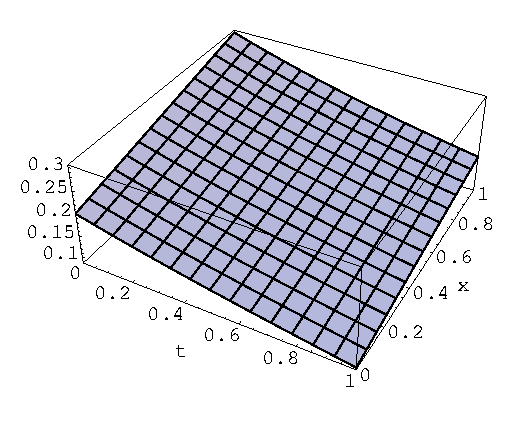
\includegraphics{senu_gr1.eps}}}
\subfigure[An example of an individual figure sub-caption.]{
\resizebox*{6cm}{!}{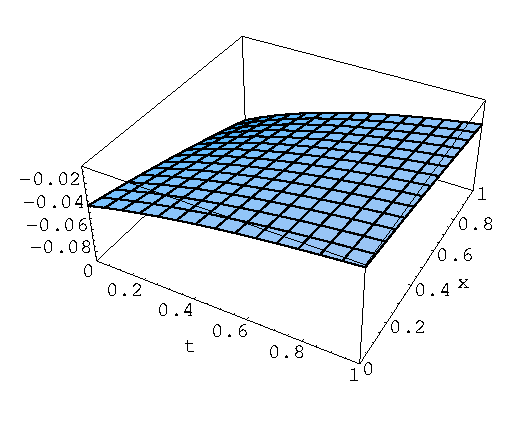
\includegraphics{senu_gr2.eps}}}
\caption{\label{fig2} Example of a two-part figure with individual 
sub-captions showing that captions are flush left and justified if 
greater than one line of text, otherwise centred under the figure.}
\label{sample-figure}
\end{center}
\end{figure}
\end{verbatim}

%\begin{figure}
%\begin{center}
%\subfigure[An example of an individual figure sub-caption.]{
%\resizebox*{6cm}{!}{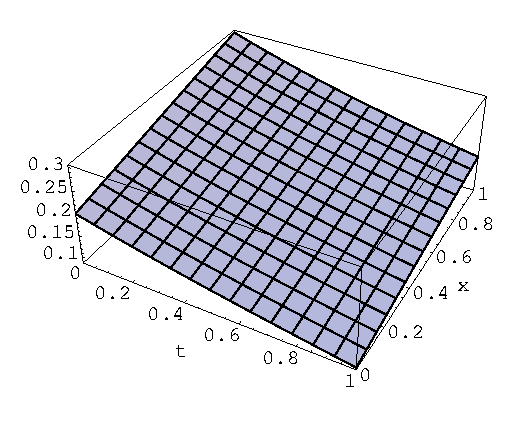
\includegraphics{senu_gr1.eps}}}\hspace{5pt}
%\subfigure[An example of an individual figure sub-caption.]{
%\resizebox*{6cm}{!}{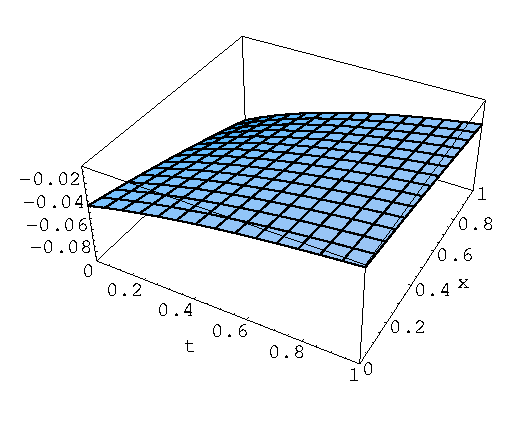
\includegraphics{senu_gr2.eps}}}
%\caption{\label{fig2} Example of a two-part figure with individual 
%sub-captions showing that captions are flush left and justified if 
%greater than one line of text, otherwise centred under the figure.}
%\label{sample-figure}
%\end{center}
%\end{figure}

The control sequences \verb"\epsfig{}", \verb"\subfigure{}" and \verb"\includegraphics{}" require epsfig.sty,
subfigure.sty and graphicx.sty. These are called by the tADR2e class file and are included with the \LaTeX\
package for this journal for convenience.

To ensure that figures are correctly numbered automatically, the \verb"\label{}" command should be inserted just
after \verb"\caption{}".


\subsection{Tables}

The {\it tADR} class file will cope with most positioning of your tables and you should not normally use the optional
positional qualifiers of the {\tt table} environment, which would override these decisions. The table caption
appears above the body of the table in {\it tADR} style, therefore the \verb"\tbl" command should appear before
the body of the table.

The {\tt tabular} environment can be used to produce tables with single thick and thin horizontal rules, which
are allowed, if desired. Thick rules should be used at the head and foot only and thin rules elsewhere.

Commands to redefine quantities such as \verb"\arraystretch" should be omitted. For example, Table~\ref{symbols}
is produced using the following commands. Note that \verb"\rm" will produce a roman character in math mode. There
are also \verb"\bf" and \verb"\it", which produce bold face and text italic in math mode.

\begin{table}
\tbl{Radio-band beaming model parameters for\\ {FSRQs and BL Lacs.}}
{\begin{tabular}[l]{@{}lcccccc}\toprule
  Class$^{\rm a}$
  & $\gamma _1$ & $\gamma _2$$^{\rm b}$
         & $\langle \gamma \rangle$
         & $G$ & $|{\bm f}|$ & $\theta _{c}$ \\
\colrule
  BL Lacs &5 & 36 & 7 & $-4.0$ & $1.0\times 10^{-2}$ & 10$^\circ$ \\
  FSRQs & 5 & 40 & 11 & $-2.3$ & $0.5\times 10^{-2}$ & 14$^\circ$ \\
\botrule
\end{tabular}}
\tabnote{$^{\rm a}$This footnote shows what footnote symbols to use.}
\tabnote{$^{\rm b}$This footnote shows the text turning over when a long footnote is added.}
\label{symbols}
\end{table}


\begin{verbatim}
\begin{table}
\tbl{Radio-band beaming model parameters for {FSRQs and BL Lacs.}}
{\begin{tabular}{@{}lcccccc}\toprule
  Class$^{\rm a}$
  & $\gamma _1$ & $\gamma _2$$^{\rm b}$
         & $\langle \gamma \rangle$
         & $G$ & $|{\bm f}|$ & $\theta _{c}$ \\
\colrule
  BL Lacs &5 & 36 & 7 & $-4.0$ & $1.0\times 10^{-2}$ & 10$^\circ$ \\
  FSRQs & 5 & 40 & 11 & $-2.3$ & $0.5\times 10^{-2}$ & 14$^\circ$ \\
\botrule
\end{tabular}}
\tabnote{$^{\rm a}$This footnote shows what footnote symbols to use.}
\tabnote{$^{\rm b}$This footnote shows the text turning over when a 
 long footnote is added.}
\label{symbols}
\end{table}
\end{verbatim}

To ensure that tables are correctly numbered automatically, the
\verb"\label{}" command should be inserted just before
\verb"\end{table}".


\subsection{Theorem-like environments}

A predefined \verb"proof" environment is provided by the {\tt amsthm} package (which is called by the class file), as follows:

\begin{proof}
More recent algorithms for solving the semidefinite programming relaxation are
particularly efficient, because they explore the structure of the MAX-CUT problem.
\end{proof}
\noindent This was produced by simply typing:
%
\begin{verbatim}
\begin{proof}
More recent algorithms for solving the semidefinite programming relaxation
are particularly efficient, because they explore the structure of the MAX-CUT
problem.
\end{proof}
\end{verbatim}
%
Other theorem-like environments (theorem, lemma, corollary, etc.) need to be defined as required, e.g. using
\verb"\newtheorem{theorem}{Theorem}" in the preamble of your .tex file before \verb"\begin{document}". The
format of the text in these environments will be changed if necessary to match the style of the journal by the
typesetter during preparation of your proofs.


\subsection{Typesetting mathematics}\label{TMth}

\subsubsection{Displayed mathematics}

The {\it tADR} class file will set displayed mathematics centred on the measure without equation numbers, provided
that you use the \LaTeXe\ standard control sequences open (\verb"\[") and close (\verb"\]") square brackets as
delimiters. The equation
\[
  \sum_{i=1}^p \lambda_i = {\rm trace}({\textrm{\bf S}})\qquad
  i\in {\mathbb R}
\]
\normalfont was typeset using the commands
%
\begin{verbatim}
\[
  \sum_{i=1}^p \lambda_i = {\rm trace}({\textrm{\bf S}})\qquad
  i\in {\mathbb R}
\].
\end{verbatim}

For those of your equations that you wish to be automatically
numbered sequentially throughout the text, use the {\tt{equation}}
environment, e.g.

\begin{equation}
  \sum_{i=1}^p \lambda_i = {\rm trace}({\textrm{\bf S}})\qquad
  i\in {\mathbb R}
\end{equation}
was typeset using the commands

\begin{verbatim}
\begin{equation}
  \sum_{i=1}^p \lambda_i = {\rm trace}({\textrm{\bf S}})quad
  i\in {\mathbb R}
\end{equation}
\end{verbatim}

Part numbers for sets of equations may be generated using the
{\tt{subequations}} environment, e.g.
\begin{subequations} \label{subeqnexample}
\begin{equation}
        \varepsilon \rho w_{tt}(s,t)
        =
        N[w_{s}(s,t),w_{st}(s,t)]_{s},
        \label{subeqnpart}
\end{equation}
\begin{equation}
        w_{tt}(1,t)+N[w_{s}(1,t),w_{st}(1,t)] = 0,
\end{equation}
\end{subequations}
which was generated using the control sequences

\begin{verbatim}
\begin{subequations} \label{subeqnexample}
\begin{equation}
        \varepsilon \rho w_{tt}(s,t)
        =
        N[w_{s}(s,t),w_{st}(s,t)]_{s},
        \label{subeqnpart}
\end{equation}
\begin{equation}
        w_{tt}(1,t)+N[w_{s}(1,t),w_{st}(1,t)] = 0,
\end{equation}
\end{subequations}
\end{verbatim}
This is made possible by the package {\tt{subeqn}}, which is called
by the class file. If you put the \verb"\label{}" just after the
\verb"\begin{subequations}" line, references will be to the
collection of equations, `(\ref{subeqnexample})' in the example
above. Or, like the example code above, you can reference each
equation individually -- e.g. `(\ref{subeqnpart})'.


\subsubsection{Bold math italic symbols}

To get bold math italic you can use \verb"\bm", which works for
all sizes, e.g.
%
\begin{verbatim}
\sffamily
\begin{equation}
   {\rm d}({\bm s_{t_{\bm u}}) = \langle{\bm\alpha({\sf{\textbf L}})}%
   [RM({\bm X}_y + {\bm s}_t) - RM({\bm x}_y)]^2 \rangle
\end{equation}
\normalfont
\end{verbatim}
%
produces\sffamily
\begin{equation}
   {\rm d}({\bm s_{t_{\bm u}}}) = \langle {\bm\alpha({\sf{\textbf L}})}[RM({\bm X}_y
   + {\bm s}_t) - RM({\bm x}_y)]^2 \rangle
\end{equation}\normalfont
Note that subscript, superscript, subscript to subscript, etc.
sizes will take care of themselves and are italic, not bold,
unless coded individually. \verb"\bm" produces the same effect as
\verb"\boldmath". \verb"\sffamily"...\verb"\normalfont" allows
upright sans serif fonts to be created in math mode by using the
control sequence `\verb"\sf"'.


\subsubsection{Bold Greek}\label{boldgreek}

Bold lowercase as well as uppercase Greek characters can be
obtained by \verb"{\bm \gamma}", which gives ${\bm \gamma}$, and
\verb"{\bm \Gamma}", which gives ${\bm \Gamma}$.


\subsubsection{Upright lowercase Greek characters and the upright partial derivative sign}\label{upgreek}

Upright lowercase Greek characters can be obtained with the class file by inserting the letter `u' in the control
code for the character, e.g. \verb"\umu" and \verb"\upi" produce $\umu$ (used, for example, in the symbol for the
unit microns -- $\umu{\rm m}$) and $\upi$ (the ratio of the circumference to the diameter of a circle). Similarly,
the control code for the upright partial derivative $\upartial$ is \verb"\upartial".

\subsection{Acknowledgements}

This unnumbered section, e.g. \verb"\section*{Acknowledgement(s)}", should be used for thanks, grant details, etc.
and placed before any Notes or References sections.

\subsection{Notes}

This unnumbered section, e.g. \verb"\section*{Note(s)}", may be placed before any References section.


\subsection{References}\label{refs}

\subsubsection{References cited in the text}

References should be cited in US National Library of Medicine (NLM) style (please see the style guide in the journal's Instructions for Authors for details). References should be cited in the text by a number in square brackets (e.g. [1], [2,4,10], [11--15], not [11]--[15]), in the order in which they first appear. Each bibliographical entry has a key, which is assigned by the author and used to refer to that entry in the text. In this document, the key \verb"neu83" in the citation form \verb"\cite{neu83}" produces `\cite{neu83}', and the keys \verb"ed84" and \verb"aiex00" in the citation form
\verb"\cite{ed84,aiex00}" produce `\cite{ed84,aiex00}'. The citation for a range of bibliographic entries (e.g.
`\cite{Eri1984,glov00,hk97,glov86,Agu95,Holl04,Maz91,Mil93}') will automatically be produced by
\verb"\cite{Eri1984,glov00,hk97,glov86,Agu95,Holl04,Maz91,Mil93}". Optional notes may be included at the end of a citation by the use of square brackets, e.g. \verb"\cite[see][p.73-–77]{cwm73}" produces `\cite[see][p.73--77]{cwm73}'.


\subsubsection{The list of references}

References should be listed at the end of the main text in the order in which they are first cited in the text. The following list shows some references prepared in the style of the journal:

\begin{thebibliography}{12}

\bibitem{neu83}
Neumann M. Parallel GRASP with path-relinking for job shop scheduling. Mol
  Phys. 1983;50:841--843.

\bibitem{ed84}
Edwards DMF, McDonald IR. Positive bases in numerical optimization. Comput
  Optim Appl. 1984;21:169--175.

\bibitem{aiex00}
Aiex RM, Pierce IF, Donizetti G, von~Weber CM, Bizet G, Bach CPE, Strauss
  R, van~Beethoven L, Mozart WA, Dukas P. Computing tools for modelling
  orchestral performance. University of Cambridge, Cambridge, UK; 2000. Tech
  Rep DAMTP 2000/NA10.

\bibitem{Eri1984}
Ericsson KA, Simon HA. Protocol analysis: verbal reports as data. Cambridge
  (MA): MIT Press; 1984.

\bibitem{glov00}
Glover F. Multi-start and strategic oscillation methods -- principles to exploit
  adaptive memory. In: Laguna M, Gonz\'{a}les-Velarde JL, editors. Computing
  tools for modeling, optimization and simulation: interfaces in computer
  science and operations research. 2nd ed. Vol.~2. Boston (MA): Kluwer Academic;
  2000. p. 1--24.

\bibitem{hk97}
Kern H. The resurgent Japanese economy and a Japan--United States free
  trade agreement. In: Lambert C, Holst G, editors. 4th International
  Conference on the Restructuring of the Economic and Political System in Japan
  and Europe. Milan, Italy, 1996 May 21--25. Singapore: World Scientific;
  1997. p. 147--156.

\bibitem{glov86}
Glover F. Hilbert modular forms and the Galois representations associated to
  Hilbert--Blumenthal abelian varieties [Ph.D. thesis]. Harvard
  University, Cambridge (MA); 1986.

\bibitem{Agu95}
Agutter AJ. The linguistic significance of current British slang [unpublished
  doctoral dissertation]. Edinburgh University, UK; 1995.

\bibitem{Holl04}
Holland M. Guide to citing internet sources. 2004~[cited~2012 Nov 4].
  Available from: http://www.bournemouth.ac.uk/library/using/guide\_to\_citing\_internet\_sourc.html.

\bibitem{Maz91}
Mazzeo J. Comparability of computer and paper-and-pencil scores (College Board
  Rep. No. 91). Princeton (NJ): Educational Testing Service; 1991.

\bibitem{Mil93}
Miller ME. The interactive tester (version 4.0) [computer software].
  Westminster (CA): Psytek Services; 1993.

\bibitem{cwm73}
Misner CW. Efficient algorithms for layer assignment problems. In: Gottlob I,
  editor. Gravitation in a collapsing Universe. 2nd ed. Vol.~5, Einstein's Legacy.
   San Francisco (CA): Freeman; 1973. p. 63--83.

\end{thebibliography}

\bigskip
\noindent This was produced by typing:
\medskip

\begin{verbatim}
\begin{thebibliography}{12}

\bibitem{neu83}
Neumann M. Parallel GRASP with path-relinking for job shop scheduling. Mol
 Phys. 1983;50:841--843.

\bibitem{ed84}
Edwards DMF, McDonald IR. Positive bases in numerical optimization. Comput
 Optim Appl. 1984;21:169--175.

\bibitem{aiex00}
Aiex RM, Pierce IF, Donizetti G, von~Weber CM, Bizet G, Bach CPE, Strauss R,
 van~Beethoven L, Mozart WA, Dukas P. Computing tools for modelling orchestral
 performance. University of Cambridge, Cambridge, UK; 2000.
 Tech Rep DAMTP 2000/NA10.

\bibitem{Eri1984}
Ericsson KA, Simon HA. Protocol analysis: verbal reports as data. Cambridge
 (MA): MIT Press; 1984.

\bibitem{glov00}
Glover F. Multi-start and strategic oscillation methods -- principles to
 exploit adaptive memory. In: Laguna M, Gonz\'{a}les-Velarde JL, editors.
 Computing tools for modeling, optimization and simulation: interfaces in
 computer science and operations research. 2nd ed. Vol.~2. Boston (MA): Kluwer
 Academic; 2000. p. 1--24.

\bibitem{hk97}
Kern H. The resurgent Japanese economy and a Japan--United States free trade
 agreement. In: Lambert C, Holst G, editors. 4th International Conference on
 the Restructuring of the Economic and Political System in Japan and Europe.
 Milan, Italy, 1996 May 21--25. Singapore: World Scientific; 1997. p. 147--156.

\bibitem{glov86}
Glover F. Hilbert modular forms and the Galois representations associated to
 Hilbert--Blumenthal abelian varieties [Ph.D. thesis]. Harvard University,
 Cambridge (MA); 1986.

\bibitem{Agu95}
Agutter AJ. The linguistic significance of current British slang [unpublished
 doctoral dissertation]. Edinburgh University, UK; 1995.

\bibitem{Holl04}
Holland M. Guide to citing internet sources. 2004 [cited~2012 Nov 4].
 Available from:
 http://www.bournemouth.ac.uk/library/using/guide\_to\_citing\_internet\_sourc.html.

\bibitem{Maz91}
Mazzeo J. Comparability of computer and paper-and-pencil scores (College Board
 Rep. No. 91). Princeton (NJ): Educational Testing Service; 1991.

\bibitem{Mil93}
Miller ME. The interactive tester (version 4.0) [computer software].
  Westminster (CA): Psytek Services; 1993.

\bibitem{cwm73}
Misner CW. Efficient algorithms for layer assignment problems. In: Gottlob I,
 editor. Gravitation in a collapsing Universe. 2nd ed. Vol.~5, Einstein's
 Legacy. San Francisco (CA): Freeman; 1973. p. 63--83.

\end{thebibliography}
\end{verbatim}
\medskip
\noindent Each entry takes the form:\vspace{12pt}

\noindent\verb"\bibitem{key}Bibliography entry"
\vspace{12pt}

\noindent where `{\tt key}' is the tag that is to be used as an argument for the \verb"\cite{}" command in the text of the article. The {\tt Bibliography entry} should be the material that is to appear in the list of references, suitably formatted.

Instead of typing the bibliography by hand, you may prefer to create the list of references using a \textsc{Bib}\TeX\ database. Include the lines \vspace{12pt}

\noindent\verb"\bibliographystyle{tADR}"
\newline\verb"\bibliography{tADRguide}"
\vspace{12pt}

\noindent where the list of references should appear, where \texttt{tADR} is the name of the \textsc{Bib}\TeX\ style file for this journal and \texttt{tADRguide} is the database of bibliographic details for the references section included with the {\itshape tADR} \LaTeX\ style package (to be replaced with the name of your own \textsc{Bib}\TeX\ database).

The \LaTeXe\ source file of your paper will extract from your .bib file only those references that are cited in that paper and list them in the References section of it.


\subsection{Appendices}\label{appendices}

Any appendices should be placed after the list of references, beginning with the
command \verb"\appendices" followed by the command \verb"\section"
for each appendix title, e.g.
%
\begin{verbatim}
\appendices
\section{This is the title of the first appendix}
\section{This is the title of the second appendix}
\end{verbatim}

\noindent produces:\medskip

\noindent Appendix A. This is the title of the first appendix

\noindent Appendix B. This is the title of the second appendix

\medskip
Subsections, equations, figures, tables, etc. within
appendices will then be automatically numbered as appropriate.


\subsection{{\bi tADR} macros}
Table~\ref{macros} gives a list of macros for use with {\it tADR}. The list displays each macro's code and a
description/demonstration of its function.

\begin{table} \tbl{{\it tADR} macros.}{\begin{tabular}{@{}ll}\toprule
$\backslash$thanks\{title-page footnote to article title & e.g. `Corresponding author. E-mail:\\
or author\} & A.N. Author@uiowa.edu'\\\cr

$\backslash$begin\{abstract\}...$\backslash$end\{abstract\} & for
abstract on titlepage\\\\ $\backslash$bm\{math and symbols\} &
bold italic $\bm{math\;and\;symbols}$\\\cr $\backslash$bi\{text\}
& bold italic \bi{text}\\\cr $\backslash$sf\{text or upright
symbols in math mode\} & sans serif \sf{text} or
$\sf{upright\;symbols\;in\;math\;mode}$
\\\botrule
\end{tabular}}
\label{macros}
\end{table}


\section{Example of a section heading including {\fontencoding{T1}\scshape{small caps}},
   {\bi italic}, and bold Greek such as ${\bm\kappa}$}\label{headings}
%
The following code shows how to achieve this section head:
%
\begin{verbatim}
\section{Example of a section heading including
{\fontencoding{T1}\scshape{small caps}}, {\bi italic},
and bold Greek such as ${\bm\kappa}$}\label{headings}
\end{verbatim}
%
%%%%%%%%%%%%%%%%%%%%%%%%%%%%%%%%%%%%

\section{{\bi tADR} journal style}

The notes given here relate to common style errors found in manuscripts, but are {\itshape not\/}
intended to be exhaustive.


\subsection{Hyphens, n-rules, m-rules and minus signs}\label{dashes}

\begin{enumerate}
\item[(i)] Hyphens (one dash in \TeX/\LaTeXe). {\it tADR} uses hyphens for compound adjectives (e.g.\ low-density gas, least-squares fit,
two-component  model) but not for complex  units  or ranges, which could become cumbersome (e.g.\ 15~km~s$^{-1}$
feature, 100--200~$\umu$m observations).

\item[(ii)] n-rules (two dashes in \TeX/\LaTeXe). These are used (a) to denote a range (e.g.\ 1.6--2.2~$\umu$m);
(b) to denote the joining of two words of equal standing (e.g.\ Kolmogorov--Smirnov  test, Herbig--Haro object);
(c) as an alternative to parentheses (e.g.\ `the results -- assuming no temperature gradient -- are indicative of \ldots').

\item[(iii)] The  m-rule (three dashes in \TeX/\LaTeXe) has no specified use in {\it tADR}.

\item[(iv)] The minus sign (one dash in \TeX/\LaTeXe) is produced
automatically in math mode by use of a single dash, e.g.
\begin{equation}
y_{i} \in \{-1, 1 \} \quad \forall i \in V,
\end{equation}
\noindent where $|-V|=A^2+B^2.$\medskip

\noindent is produced by

\begin{verbatim}
\begin{equation}
y_{i} \in \{-1, 1 \} \quad \forall i \in V,
\end{equation}
\noindent where $|-V|=A^2+B^2.$
\end{verbatim}

\end{enumerate}


\subsection{References}

It is important to use the correct reference style, details  of which can be found in Section~\ref{refs} above.


\subsection{Maths fonts}

Scalar  variables should be mediumface italic (e.g. $s$ for
speed); vectors should be bold italic (e.g. $\bm v$ for velocity);
matrices should be bold roman (upright) (e.g. $\bf A$), and
tensors should be bold upright sans serif (e.g. {\sffamily{\textbf
L}}). Differential d, partial differential $\upartial$, complex i,
exponential e, superscript T for `transpose', sin, cos, tan, log,
etc., should all be roman. Openface, or `blackboard', fonts can be
used, for example, for the integers $\mathbb Z$ and the reals
$\mathbb R$. Sub/superscripts that are physical variables should
be italic, while those  that are labels should be roman (e.g.\
$C_p$, $T_{\rm eff}$). Displayed equations should have end-of-line
punctuation appropriate to the running text sentence of which they
form a part.


\section{Troubleshooting}

Authors may from time to time encounter problems with the  preparation
of their papers in \LaTeX\/. The appropriate  action  to
take will depend on the nature of the problem -- the following is
intended to act as a guide.
%
\begin{enumerate}
\item[(i)] If the problem is with \LaTeX\ itself, rather than with the
actual macros, please refer to the appropriate handbooks for
initial advice.\footnote{\TeX: Knuth, D., 1986, {\it The \TeX\
book} (New York: Addison--Wesley); \LaTeXe: Lamport, L., 1994,
{\it \LaTeX: A Document Preparation System}, 2nd edn (New
York: Addison--Wesley).} If the solution cannot be found, and you
suspect that the problem lies with the macros, then please contact
Taylor \& Francis ({\tt latex.helpdesk@tandf.co.uk}).

\item[(ii)] Problems with page make-up (e.g.\ large spaces between paragraphs, or under headings or
figures; uneven columns; figures/tables appearing out of order):
please do {\itshape not\/} attempt to remedy these yourself using
`hard' page make-up commands -- the typesetter will correct such
problems. (You may, if you wish, draw attention to particular
problems when submitting the final version of your paper.)

\item[(iii)] If a required font is not available at your site, allow \TeX\
to substitute the font and specify which font you require in the
covering letter accompanying your file(s).
\end{enumerate}


\section{Fixes for coding problems}

This guide has been designed to minimize the need for user-defined macros to  create special symbols. Authors
are urged, wherever possible, to use the following coding rather than to create their own. This will minimize
the danger of author-defined macros being accidentally `overridden' when the paper is typeset (see
Section~\ref{TMth}, `Typesetting mathematics'). In cases where it is essential to create your own macros,
these should be displayed in the preamble of the source file before \verb"\begin{document}".

%
\begin{enumerate}
\item[(i)] Fonts in section headings and paper titles. The following are  examples
of styles that sometimes prove difficult to code.


\subsection*{Paper titles:}

\hsize380pt\bf{\noindent Generalized Flory theory at ${\bm\delta >
{\bf
   50}^\circ}$}\\

    \noindent\normalfont is produced by
\begin{verbatim}
\title{Generalized Flory theory at
        ${\bm\delta > {\bfseries 50}^\circ}$}
\end{verbatim}
\bigskip

{\bf{\noindent Ion--ion correlations in H\,{\sc ii} regions}}\\

\noindent\normalfont is produced by
%
\begin{verbatim}
\title{Ion--ion correlations in H\,{\sc ii} regions}
\end{verbatim}


\stepcounter{enumi}

\item[(ii)] n-rules, m-rules, hyphens and minus signs (see Section~\ref{dashes} for
correct usage). To create the correct symbols in the sentence
%
\begin{quote}
The high-resolution observations were made along a line at an
angle of $-15^\circ$ (East from North) from the axis of the
jet -- which runs North--South
\end{quote}
you would use the following code:
%
\begin{verbatim}
The high-resolution observations were made along a line at an angle
of $-15^\circ$ (East from North) from the axis of the jet -- which
runs North--South
\end{verbatim}

\item[(iii)] Fonts in superscripts and subscripts. Subscripts and superscripts will automatically come  out in the correct font
and size in a math environment (e.g. enclosed by `\verb"$"'
delimiters in running text or within \verb"\[...\]" or the
`equation' environment for displayed equations). You can create
the output ${\bm k_x}$ by typing \verb"${\bm k_x}$". If the
subscripts or superscripts need to be other than italic, they
should be coded individually -- see (vi) below.

\item[(iv)] Calligraphic letters (uppercase only).
%
Normal calligraphic can be produced with \verb"\cal" as usual (in
math mode).

\item[(v)] Automatic scaling of brackets. The codes \verb"\left" and
\verb"\right" should  be used to scale brackets automatically to
fit the equation being set. For example, to get
\[
   v = x \left( \frac{N+2}{N} \right)
\]
use the code
%
\begin{verbatim}
\[
   v = x \left( \frac{N+2}{N} \right)
\]
\end{verbatim}

\item[(vi)] Roman font in equations. It is often necessary to make some
symbols roman in an equation (e.g.\ units, non-variable
subscripts). For example, to get
\[
   \sigma \simeq (r/13~h^{-1}~{\rm Mpc})^{-0.9},
   \qquad \omega = \frac{N-N_{\rm s}}{N_{\rm R}}
\]
\noindent use the code:
%
\begin{verbatim}
\[
   \sigma \simeq (r/13~h^{-1}
   ~{\rm Mpc})^{-0.9}, \qquad \omega
   =\frac{N-N_{{\rm s}}}{N_{{\rm R}}}
\]
\end{verbatim}
The {\tt siunits} package of macros for typesetting units is also compatible with the {\it tADR} class file.
\end{enumerate}


\section{Obtaining the tADR2e class file}\label{FTP}

\subsection{Via the Taylor \& Francis website}

This Guide for Authors and the tADR2e.cls class file may be obtained via the Instructions for Authors
on the Taylor \& Francis homepage for the journal.

Please note that the class file calls up the following open-source \LaTeX\ packages, which will, for convenience,
unpack with the downloaded Guide for Authors and class file: amsbsy.sty; amsfonts.sty; amsmath.sty; amssymb.sty; epsfig.sty; graphicx.sty; natbib.sty; rotating.sty; subfigure.sty.

\subsection{Via e-mail}

This Guide for Authors, the class file and the associated open-source \LaTeX\ packages are also available by
e-mail. Requests should be addressed to {\tt latex.helpdesk@tandf.co.uk} clearly stating for which journal you
require the Guide for Authors and/or class file.

\label{lastpage}

\end{document}
